\chapter{Related Work}
\section{Reference Games}
Although, the idea of communication as a signaling game goes back to \cite{Lewis_1969}, we will be focusing on a type of a signaling game called a reference gam, as presented in \cite{Frank_2012}. The game tries to mimic the challenges of communication that people face on daily basis, as we discussed in the introduction. At first, an instance of a reference game looked as in \autoref{fig:intro_complex}, that is, no information about the available messages is given to the speaker and listener. The later instances, on the other hand, include this information. The examples are shown in \autoref{fig:simple_complex}. The goal for newer version is the same, that is, to identify which object a speaker is referring to. This change allows for more controlled experiments by increasing the variability in setups. In addition, it should improve clarity, for instance, participants should not wonder, why wouldn't the speaker just utter the location of the object instead of specifying the properties.

\begin{figure}
\centering
\begin{subfigure}{.5\textwidth}
  \centering
  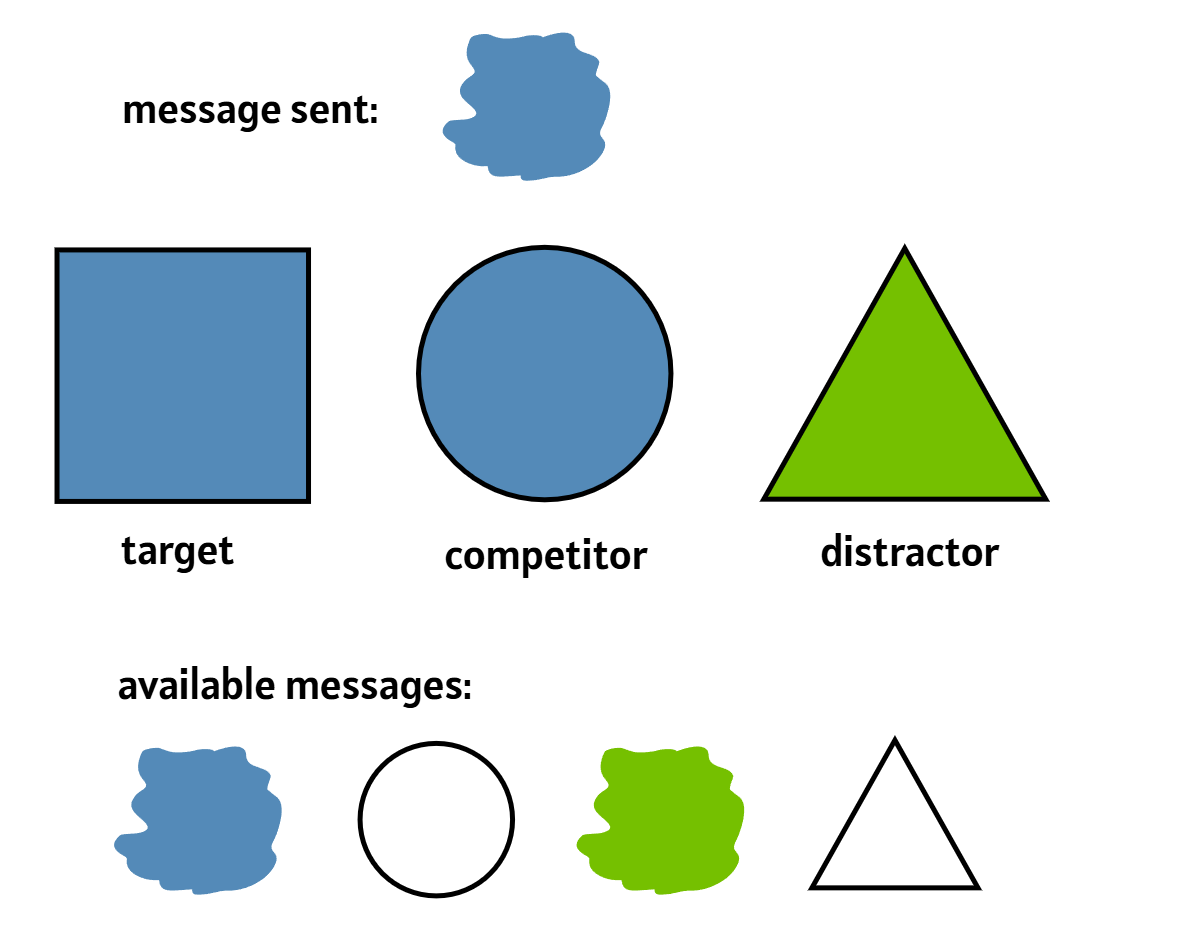
\includegraphics[width=1\linewidth]{images/simple.png}
  \caption{Simple}
  \label{fig:simple}
\end{subfigure}%
\begin{subfigure}{.5\textwidth}
  \centering
  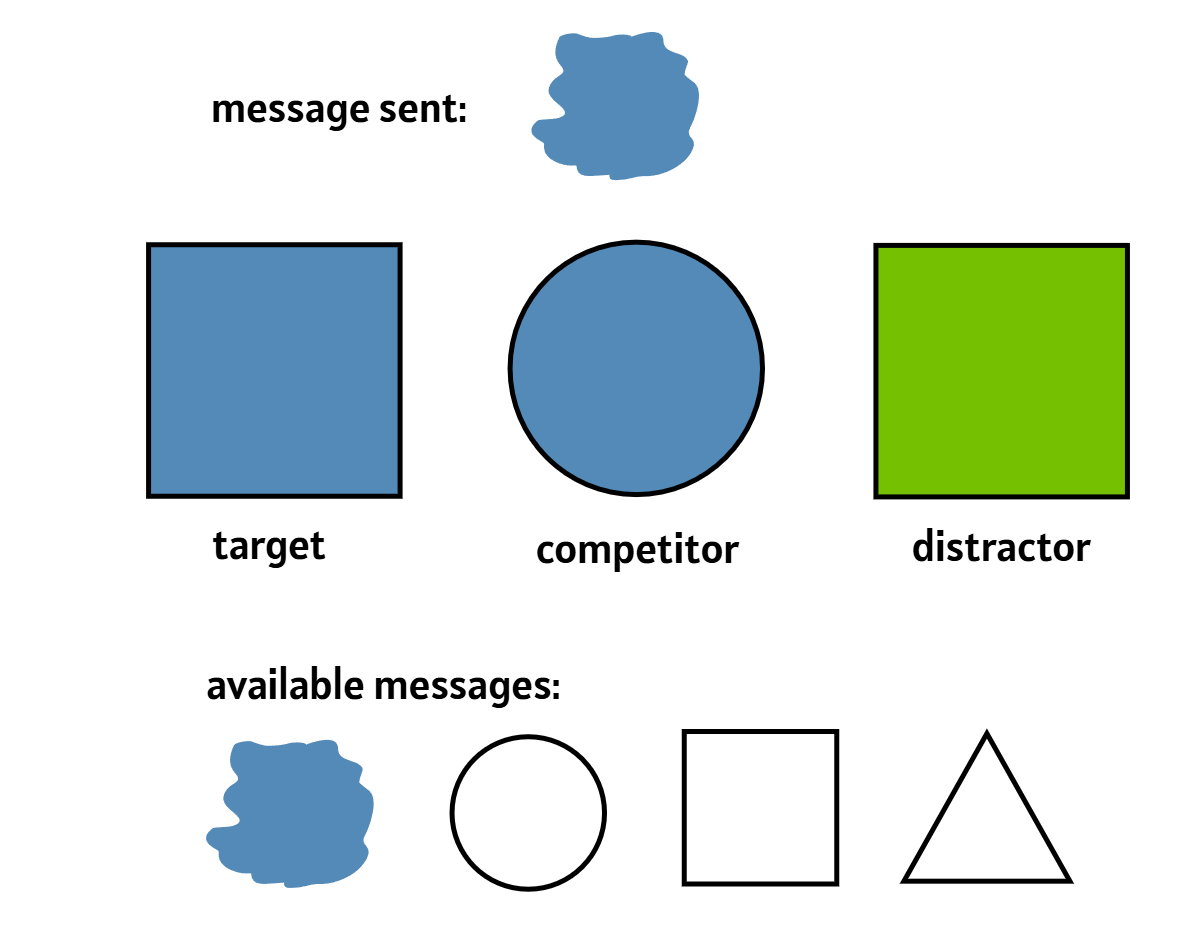
\includegraphics[width=1\linewidth]{images/complex.png}
  \caption{Complex}
  \label{fig:complex}
\end{subfigure}
\caption{Two instances of reference games with different difficulties. }
\label{fig:simple_complex}
\end{figure}

Let's take a closer look at \autoref{fig:simple}. An uttered message is presented on the top. We will denote the object being referred to as a Target, a Competitor is an object that shares the message property with the Target. While a Disctractor does not share the sent message property, but could share another property with the Target depending on the difficulty of the trial. Note that, obviously, captions Target, Competitor and Disctractor are not available to the participants. The difference between the Simple and Complex trials in \autoref{fig:simple_complex} mainly in how the Disctractor is constructed. In particular, in the Simple trial it does not share any properties with the Target, while in the Complex it does. The Simple example \autoref{fig:simple} can be solved without considering the Disctractor. That is, one could count the matching messages from the available ones. In this case, it would be 1 for blue square, 2 for blue circle and 2 for green triangle. Hence, the Target is blue square, as ``blue'' is the only message that could refer to it. This way of solving is not necessarily what people tend to do, but it is one way of interpreting the difference between Simple and Complex trials. Because if you apply the same strategy to the Complex example in \autoref{fig:complex}, both Target and Competitor have two matching messages. On the other hand, if you try to solve these examples yourself, you will probably end up recursively reasoning of what the speaker could have said had they had another Target. The Simple and Complex in this case still appear to their names, you will need a more robust recursion in order to solve the Complex one comparing to the Simple one.

\section{Rational Speech Act Model} \label{sec:rsa}
Studying this phenomena needs a formalized approach. One such model, called the Rational Speech Act (RSA) was developed. It mimics how a speaker and a listener reason about each other. A detailed explanation can be found in the manuscript by \cite{Frank_2016} as well as in the article by \cite{Franke_2016}. We will go through the main ideas on how a listener and a speaker interact with each other. Firstly, take a look at the matrix $M_s$ from the \autoref{eq:1}. Each column is a one-hot encoding of an objects, in other words this matrix encodes which objects match the literal meaning of each message, this matrix is constructed for the Simple example in \autoref{fig:simple}. 
\begin{equation} \label{eq:1}
M_s = \!\!\!\!
\raisebox{2.3ex}{$
\begin{array}{c@{\;}c}
    & {
    \begin{array}{*{4}{C{20pt}}} 
        \inlinegraphics{images/shapes_and_colors/blue_square.png} & \inlinegraphics{images/shapes_and_colors/blue_circle.png} & \inlinegraphics{images/shapes_and_colors/green_triangle.png}  
      \end{array}} \\[5pt]
    \begin{array}{c} 
        \inlinegraphics{images/shapes_and_colors/blue.png} \\ 
        \inlinegraphics{images/shapes_and_colors/circle.png} \\ 
        \inlinegraphics{images/shapes_and_colors/green.png} \\
        \inlinegraphics{images/shapes_and_colors/triangle.png}
    \end{array} 
    & 
    \left[
    \begin{array}{*{3}{C{20pt}}}
        1 & 1 & 0  \\
        0 & 1 & 0  \\
        0 & 0 & 1  \\
        0 & 0 & 1  \\
    \end{array} \right]
\end{array}$
}
\end{equation}

Now let us give an explication for a listener matrix, each row shows conditional probabilities for an objects given a message. Accordingly, a speaker matrix has columns that depict conditional probabilities of messages given an object. 

Subsequently we arrive at a literal listener \autoref{eq:2} and speaker \autoref{eq:3}. Simply put, a literal speaker would output one of the matching messages with equal probability for the given Target. For example, if green triangle is provided for the speaker, they would refer to it by uttering ``green'' or ``triangle'' with equal probability. While literal listener would interpret the ambiguous messages with equal probabilities.

\begin{equation} \label{eq:2}
L_0(M_s)=L(M_s) =\!\!\!\!
\raisebox{2.3ex}{$
\begin{array}{c@{\;}c}
    & {
    \begin{array}{*{3}{C{20pt}}} 
        \inlinegraphics{images/shapes_and_colors/blue_square.png} & \inlinegraphics{images/shapes_and_colors/blue_circle.png} & \inlinegraphics{images/shapes_and_colors/green_triangle.png}  
      \end{array}} \\[5pt]
    \begin{array}{c} 
        \inlinegraphics{images/shapes_and_colors/blue.png} \\ 
        \inlinegraphics{images/shapes_and_colors/circle.png} \\ 
        \inlinegraphics{images/shapes_and_colors/green.png} \\
        \inlinegraphics{images/shapes_and_colors/triangle.png}
    \end{array} 
    & 
    \left[
    \begin{array}{*{3}{C{20pt}}}
        0.5 & 0.5 & 0  \\
        0 & 1 & 0  \\
        0 & 0 & 1  \\
        0 & 0 & 1  \\
    \end{array} \right]
\end{array}$
}
\end{equation}

\begin{equation} \label{eq:3}
S_0(M_s)=S(M_s) = \!\!\!\!
\raisebox{2.3ex}{$
\begin{array}{c@{\;}c}
    & {
    \begin{array}{*{4}{C{20pt}}} 
        \inlinegraphics{images/shapes_and_colors/blue_square.png} & \inlinegraphics{images/shapes_and_colors/blue_circle.png} & \inlinegraphics{images/shapes_and_colors/green_triangle.png}  
      \end{array}} \\[5pt]
    \begin{array}{c} 
        \inlinegraphics{images/shapes_and_colors/blue.png} \\ 
        \inlinegraphics{images/shapes_and_colors/circle.png} \\ 
        \inlinegraphics{images/shapes_and_colors/green.png} \\
        \inlinegraphics{images/shapes_and_colors/triangle.png}
    \end{array} 
    & 
    \left[
    \begin{array}{*{3}{C{20pt}}}
        1 & 0.5 & 0  \\
        0 & 0.5 & 0  \\
        0 & 0 & 0.5  \\
        0 & 0 & 0.5  \\
    \end{array} \right]
\end{array}$
}
\end{equation}

One could see that such approach would not solve even a Simple trial. However, if there is a completely unambiguous message, the literal listener would be able to correctly identify the Target. The way we derived the two matrices is just a normalization within columns or rows, correspondingly for the listener and speaker.  We can keep applying this technique recursively, to find more complex listeners and speakers. That is, a speaker would normalize within columns the matrix previously normalized within rows. In this way we can derive an $L_1$ listener \autoref{eq:4}, also called a first-order cooperative listener. Note that \cite{Frank_2016} and \cite{Franke_2016} apply different strategies to construct $L_1$ and $L_2$ listeners, we will stick to the \cite{Franke_2016} variation.

\begin{equation} \label{eq:4}
L_1(M_s)=L(S(M_s)) = \!\!\!\!
\raisebox{2.3ex}{$
\begin{array}{c@{\;}c}
    & {
    \begin{array}{*{4}{C{20pt}}} 
        \inlinegraphics{images/shapes_and_colors/blue_square.png} & \inlinegraphics{images/shapes_and_colors/blue_circle.png} & \inlinegraphics{images/shapes_and_colors/green_triangle.png}  
      \end{array}} \\[5pt]
    \begin{array}{c} 
        \inlinegraphics{images/shapes_and_colors/blue.png} \\ 
        \inlinegraphics{images/shapes_and_colors/circle.png} \\ 
        \inlinegraphics{images/shapes_and_colors/green.png} \\
        \inlinegraphics{images/shapes_and_colors/triangle.png}
    \end{array} 
    & 
    \left[
    \begin{array}{*{3}{C{20pt}}}
        0.66 & 0.33 & 0  \\
        0 & 1 & 0  \\
        0 & 0 & 1  \\
        0 & 0 & 1  \\
    \end{array} \right]
\end{array}$
}
\end{equation}

$L_1$ listener gives the highest probability to the Target with message blue. Repeating this procedure further to get to deeper recursion increases the probability of Target being chosen. In addition, RSA model has a greed parameter $\alpha$ which amplifies the probabilities. $\alpha=\infty$ would result in simply choosing the object with the highest probability. Now let's take a look at the Complex case and see how it differs from the Simple one. The matrix $M_c$ is given in \autoref{eq:5}.

\begin{equation} \label{eq:5}
M_c = \!\!\!\!
\raisebox{2.3ex}{$
\begin{array}{c@{\;}c}
    & {
    \begin{array}{*{4}{C{20pt}}} 
        \inlinegraphics{images/shapes_and_colors/blue_square.png} & \inlinegraphics{images/shapes_and_colors/blue_circle.png} & \inlinegraphics{images/shapes_and_colors/green_square.png}  
      \end{array}} \\[5pt]
    \begin{array}{c} 
        \inlinegraphics{images/shapes_and_colors/blue.png} \\ 
        \inlinegraphics{images/shapes_and_colors/circle.png} \\ 
        \inlinegraphics{images/shapes_and_colors/square.png} \\
        \inlinegraphics{images/shapes_and_colors/triangle.png}
    \end{array} 
    & 
    \left[
    \begin{array}{*{3}{C{20pt}}}
        1 & 1 & 0  \\
        0 & 1 & 0  \\
        1 & 0 & 1  \\
        0 & 0 & 0  \\
    \end{array} \right]
\end{array}$
}
\end{equation}

Going through the same steps to derive the $L_1$ listener, we get \autoref{eq:6}. 

\begin{equation} \label{eq:6}
L_1(M_c) = L(S(M_c)) = \!\!\!\!
\raisebox{2.3ex}{$
\begin{array}{c@{\;}c}
    & {
    \begin{array}{*{3}{C{20pt}}} 
        \inlinegraphics{images/shapes_and_colors/blue_square.png} & \inlinegraphics{images/shapes_and_colors/blue_circle.png} & \inlinegraphics{images/shapes_and_colors/green_square.png}  
      \end{array}} \\[5pt]
    \begin{array}{c} 
        \inlinegraphics{images/shapes_and_colors/blue.png} \\ 
        \inlinegraphics{images/shapes_and_colors/circle.png} \\ 
        \inlinegraphics{images/shapes_and_colors/square.png} \\
        \inlinegraphics{images/shapes_and_colors/triangle.png}
    \end{array} 
    & 
    \left[
    \begin{array}{*{3}{C{20pt}}}
        0.5 & 0.5 & 0  \\
        0 & 1 & 0  \\
        0.33 & 0 & 0.66  \\
        0 & 0 & 0  \\
    \end{array} \right]
\end{array}$
}
\end{equation}

One important difference is that depth of recursion for the $L_1$ listener is not enough to assign the highest probability to the Target. Here, the ``blue'' row has the same probabilities for the Disctractor and the Target. Note that in this case the greed parameter $\alpha$ would not be able to help. So instead we consider a deeper level of recursion and introduce an $L_2$ listener \autoref{eq:7}, also called second-order cooperative listener. 

\begin{equation} \label{eq:7}
L_2(M_c) = L(S(L(M_c))) = \!\!\!\!
\raisebox{2.3ex}{$
\begin{array}{c@{\;}c}
    & {
    \begin{array}{*{4}{C{20pt}}} 
        \inlinegraphics{images/shapes_and_colors/blue_square.png} & \inlinegraphics{images/shapes_and_colors/blue_circle.png} & \inlinegraphics{images/shapes_and_colors/green_square.png}  
      \end{array}} \\[5pt]
    \begin{array}{c} 
        \inlinegraphics{images/shapes_and_colors/blue.png} \\ 
        \inlinegraphics{images/shapes_and_colors/circle.png} \\ 
        \inlinegraphics{images/shapes_and_colors/square.png} \\
        \inlinegraphics{images/shapes_and_colors/triangle.png}
    \end{array} 
    & 
    \left[
    \begin{array}{*{3}{C{20pt}}}
        0.6 & 0.4 & 0  \\
        0 & 1 & 0  \\
        0.33 & 0 & 0.66  \\
        0 & 0 & 0  \\
    \end{array} \right]
\end{array}$
}
\end{equation}

\begin{figure}
\centering
\begin{subfigure}{.5\textwidth}
  \centering
  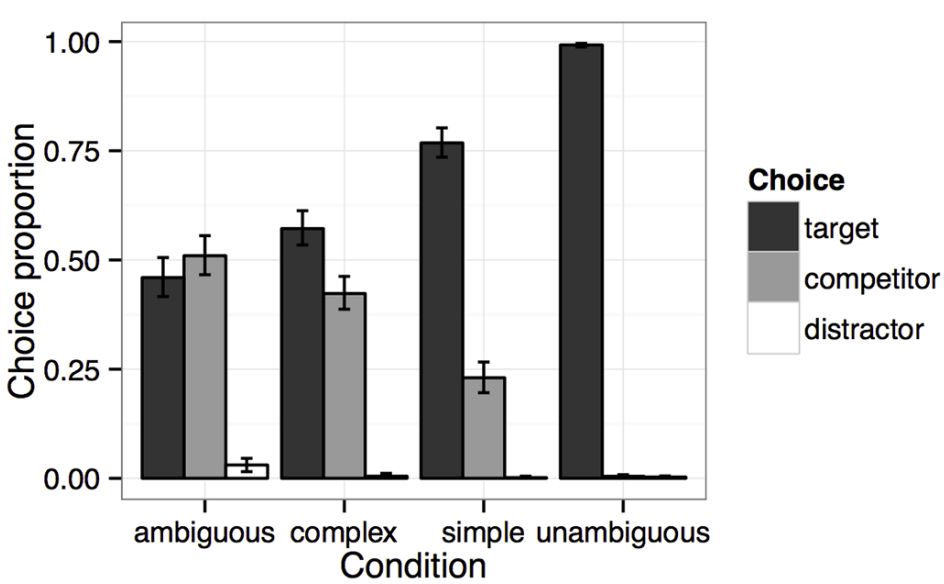
\includegraphics[width=1\linewidth]{images/trials_stats.png}
  \caption{Proportions of Target, Competitor and Disctractor choices in their experiment. }
  \label{fig:trial_stats}
\end{subfigure}%
\begin{subfigure}{.5\textwidth}
  \centering
  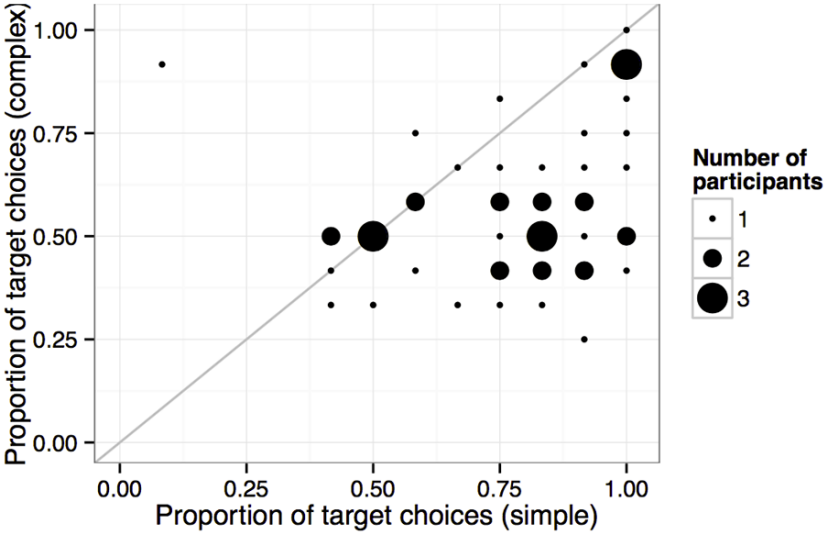
\includegraphics[width=1\linewidth]{images/l1_l2_stats.png}
  \caption{Proportion of Target choices in Simple and Complex conditions by participant. }
  \label{fig:prob_stats}
\end{subfigure}
\caption{Plots from \cite{Franke_2016}.}
\label{fig:stats}
\end{figure}

So, as one can see, the $L_2$ can correctly identify the Target considering the highest probability. Hence, the main point to take from here is that $L_1$ listener can solve the Simple task, but cannot solve the Complex one, while the $L_2$ listener is able to solve both. 

Further expending on this, the previous research shows, that the modeled listeners align with the empirical data. In particular, see \autoref{fig:stats} taken from \cite{Franke_2016}. \autoref{fig:trial_stats} shows that indeed the difficulty gets harder going from Unambiguous to Simple and further to Complex trials. On the other hand, \autoref{fig:prob_stats} shows that there are roughly 3 clusters present depending on whether one can solve only Simple, both or neither of conditions. This strongly supports the alignment with $L_0,L_1$ and $L_2$ listeners. However, very important to note that we are only talking about the alignment of RSA model's accuracy with the empirical data, while the concrete strategies are not taken into account.

Now we will proceed further, and make a hypothesis about how people could be solving these problems. A key difference between Simple and Complex trials is the fact that solving Complex trials requires one to consider the Disctractor as well due to the matching feature with the Target, while in the Simple one, the Disctractor can be ignored completely. This can be demonstrated by the following matrix transformations. If one does not take into account the Disctractor the $M_s,M_c$ will instead look as in \autoref{eq:8} and \autoref{eq:9} correspondingly. 

\begin{equation} \label{eq:8}
M_s' = \!\!\!\!
\raisebox{2.3ex}{$
\begin{array}{c@{\;}c}
    & {
    \begin{array}{*{4}{C{20pt}}} 
        \inlinegraphics{images/shapes_and_colors/blue_square.png} & \inlinegraphics{images/shapes_and_colors/blue_circle.png}  
      \end{array}} \\[5pt]
    \begin{array}{c} 
        \inlinegraphics{images/shapes_and_colors/blue.png} \\ 
        \inlinegraphics{images/shapes_and_colors/circle.png} \\ 
        \inlinegraphics{images/shapes_and_colors/green.png} \\
        \inlinegraphics{images/shapes_and_colors/triangle.png}
    \end{array} 
    & 
    \left[
    \begin{array}{*{2}{C{20pt}}}
        1 & 1  \\
        0 & 1  \\
        0 & 0  \\
        0 & 0  \\
    \end{array} \right]
\end{array}$
}
\end{equation}

\begin{equation} \label{eq:9}
M_c' = \!\!\!\!
\raisebox{2.3ex}{$
\begin{array}{c@{\;}c}
    & {
    \begin{array}{*{4}{C{20pt}}} 
        \inlinegraphics{images/shapes_and_colors/blue_square.png} & \inlinegraphics{images/shapes_and_colors/blue_circle.png}
      \end{array}} \\[5pt]
    \begin{array}{c} 
        \inlinegraphics{images/shapes_and_colors/blue.png} \\ 
        \inlinegraphics{images/shapes_and_colors/circle.png} \\ 
        \inlinegraphics{images/shapes_and_colors/square.png} \\
        \inlinegraphics{images/shapes_and_colors/triangle.png}
    \end{array} 
    & 
    \left[
    \begin{array}{*{3}{C{20pt}}}
        1 & 1 \\
        0 & 1 \\
        1 & 0 \\
        0 & 0 \\
    \end{array} \right]
\end{array}$
}
\end{equation}

Applying $L_1$ transformation to the $M_s'$ we get \autoref{eq:10} which accomplishes the same as in \autoref{eq:4}.

\begin{equation} \label{eq:10}
L_1(M_s') = \!\!\!\!
\raisebox{2.3ex}{$
\begin{array}{c@{\;}c}
    & {
    \begin{array}{*{4}{C{20pt}}} 
        \inlinegraphics{images/shapes_and_colors/blue_square.png} & \inlinegraphics{images/shapes_and_colors/blue_circle.png}  
      \end{array}} \\[5pt]
    \begin{array}{c} 
        \inlinegraphics{images/shapes_and_colors/blue.png} \\ 
        \inlinegraphics{images/shapes_and_colors/circle.png} \\ 
        \inlinegraphics{images/shapes_and_colors/green.png} \\
        \inlinegraphics{images/shapes_and_colors/triangle.png}
    \end{array} 
    & 
    \left[
    \begin{array}{*{2}{C{20pt}}}
        0.66 & 0.33  \\
        0 & 1  \\
        0 & 0  \\
        0 & 0  \\
    \end{array} \right]
\end{array}$
}
\end{equation}

On the other hand, neither $L_1$ nor $L_2$ can solve the matrix $M_c'$. In fact, no depth of recursion is helpful in this case as $L_0(M_c')=L_1(M_c')=L_2(M_c')$ (\autoref{eq:11}).

\begin{equation} \label{eq:11}
L(M_c') = L(S(M_c')) = L(S(L(M_c'))) = \!\!\!\!
\raisebox{2.3ex}{$
\begin{array}{c@{\;}c}
    & {
    \begin{array}{*{4}{C{20pt}}} 
        \inlinegraphics{images/shapes_and_colors/blue_square.png} & \inlinegraphics{images/shapes_and_colors/blue_circle.png}
      \end{array}} \\[5pt]
    \begin{array}{c} 
        \inlinegraphics{images/shapes_and_colors/blue.png} \\ 
        \inlinegraphics{images/shapes_and_colors/circle.png} \\ 
        \inlinegraphics{images/shapes_and_colors/square.png} \\
        \inlinegraphics{images/shapes_and_colors/triangle.png}
    \end{array} 
    & 
    \left[
    \begin{array}{*{3}{C{20pt}}}
        0.5 & 0.5 \\
        0 & 1 \\
        1 & 0 \\
        0 & 0 \\
    \end{array} \right]
\end{array}$
}
\end{equation}

This leads us to a research question of whether people achieve $L_1$ accuracy by not considering the Disctractor and applying reasoning deeper than one of a literal speaker. Or they include the Disctractor in their reasoning but simply lack the depth of recursion therefore failing to solve the Complex trials.




\section{How Eye Tracking is Useful}
\begin{figure}
    \centering
    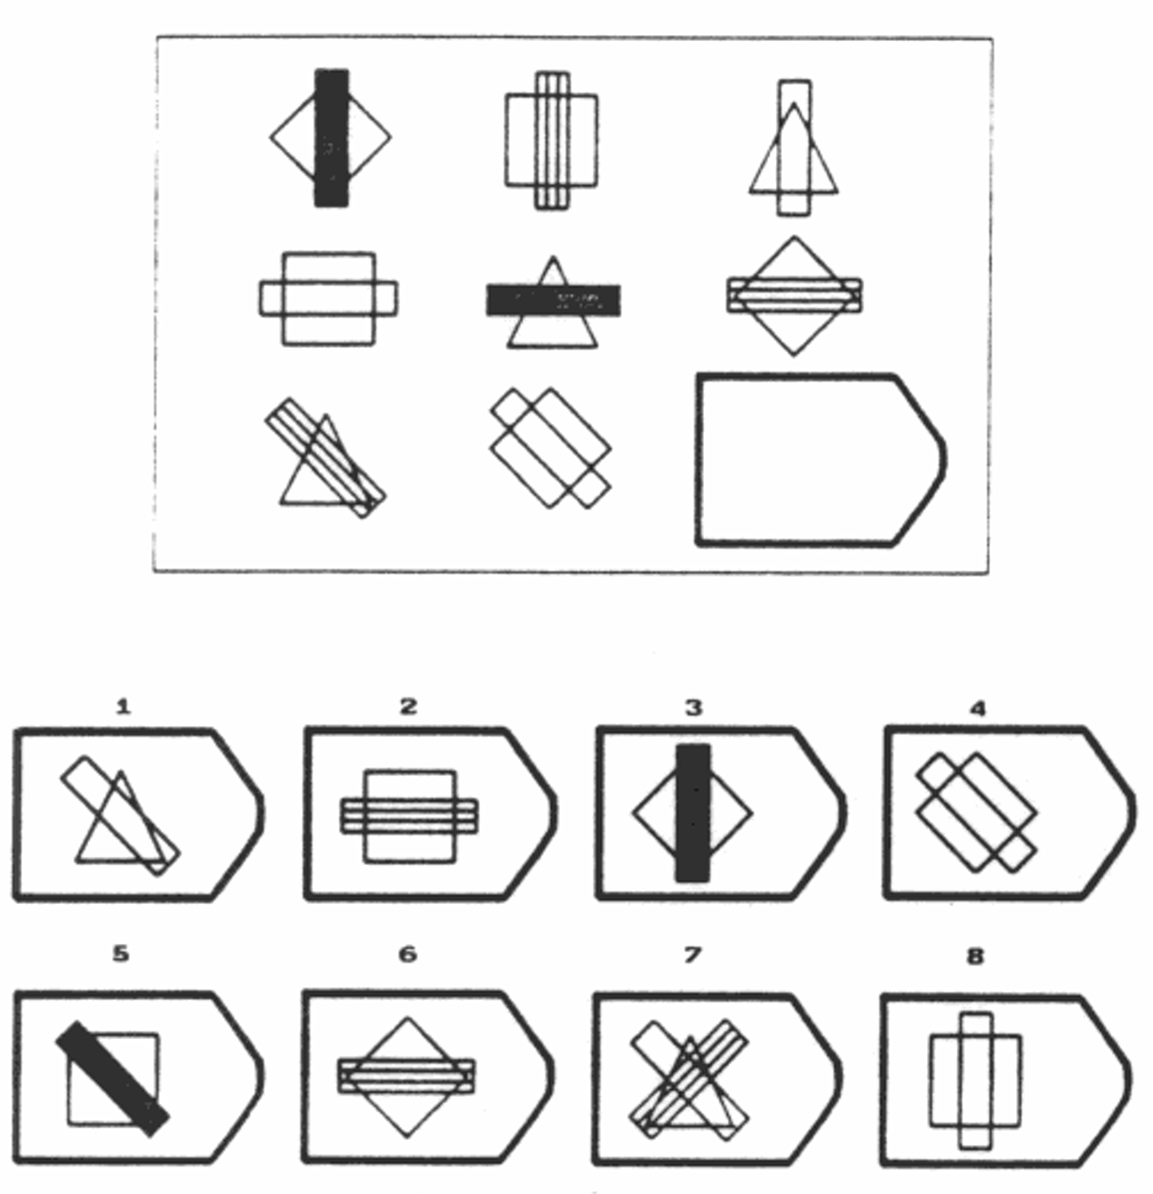
\includegraphics[width=0.5\linewidth]{images/raven_carpenter_1990.png}
    \caption{An example of Raven Test. The upper part is the matrix, while the bottom is possible answers. The matrix is constructed as follows. The lines orientation is constant within rows. While the shapes and line appearances are obeying the distribution-of-three-values rule. Simply put, same three values are present in each row. The correct answer is 5.}
    \label{fig:raven}
\end{figure}
We will take a look at a related field with different kind of tasks, this strategy has shown to be particularly informative and insightful there. 
The Raven Progressive Matrices, commonly referred to as the Raven Tests, are a set of nonverbal intelligence tests designed to measure abstract reasoning and problem-solving abilities through pattern recognition and logical inference. Such test usually contains 8 objects arranged in a 3 by 3 grid with one object missing, as well as the set of possible answers displayed below the matrix. Each matrix either has a particular rule it is constructed by or a mix of them. An example is presented in \autoref{fig:raven}. 

Researches suggest that there are two main strategies for solving the Raven Tests constructive matching and response elimination \citep{Bethel-Fox_1984} and later followed by \cite{Vigneau_2006}. The former is described as successively finding rules by which the matrix is constructed, until the answer is fully derived. And the later means that rather than going through the matrix, one goes over the possible answers and eliminates them one by one, ending up with the correct one in the end. The less efficient of these, response elimination, seemed to be used more by lower ability subjects on more difficult items. 

The two strategies can be identified by the patterns of one's attention, hence, eye gaze. The constructive matching being focused on the matrix and systematically going through rows and columns of it. \cite{Carpenter_1990} expand on the eye tracking experiments in this research question by recording eye gaze as well as the verbal comments during the process of solving the tasks. A very detailed sequence of actions is acquired, therefore, giving an insight into how one uses the constructive matching strategy to solve Raven Progressive Matrices. On the other hand, the response elimination involves a lot of toggling between the possible answers and the matrix. In order to deepen the understanding in this problem \cite{Vigneau_2006} develop a set of features to encode ones attention. Such features include for example Time on Matrix, Time on Alternatives (possible answers) or Number of Toggles between the possible answers and the matrix. The authors proceed to report the correlation between the features and the proportion of correct answers. Indeed, the results show statistically significant negative correlation of Time on Alternatives and Number of Toggles with overall score. These findings further support theory about the difference in effectiveness in the two strategies. 


One can see, based on these studies, why and how the eye tracking can be useful in the reference games. In our case as discussed in the end of \autoref{sec:rsa} there are multiple ways people could reach $L_1$ accuracy. Therefore suggesting that the two potential strategies would be distinguished by the use of Disctractor. At the same time, there are still $L_0$ and $L_2$ listeners present in the experiment which makes the distinction more difficult. On the other hand, as there is no previous work on eye tracking reference games, the study is also highly exploratory.

\section{Out of Lab Eye Tracking} \label{sec:eyetr}
\begin{figure}
    \centering
    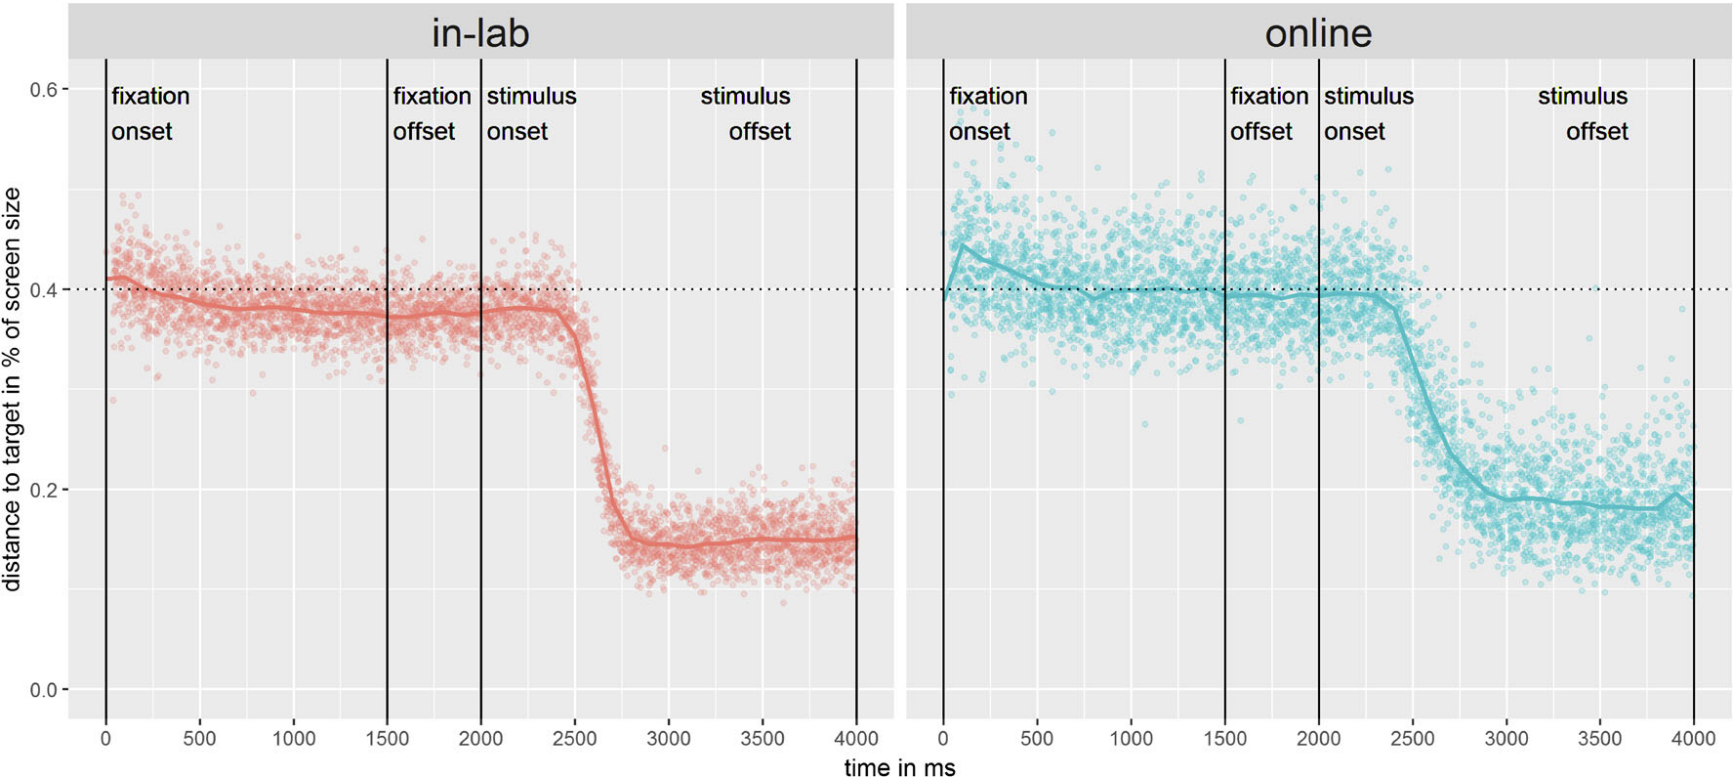
\includegraphics[width=1\linewidth]{images/tracker_comparison.png}
    \caption{Figure from \cite{Semmelmann_2018}. Fixation task results. Each dot denotes a single recorded data point in distance to a target in percentage of screen size over time.}
    \label{fig:eyetr_comparison}
\end{figure}
Up until now, most of the eye tracking studies have been using the laboratory equipment in order to conduct the experiments. This is very important as a reliable and precise method is needed for such experiments. On the other hand, this approach requires people to be physically present in the laboratory, which makes the experiment far more difficult to conduct in comparison to participants answering a series of questions on their laptops. Hence, a different approach was chosen. This experiment will incorporate participants' webcams to collect the eye tracking part of the data. In particular, a library called WebGazer will be used \citep{webgazer}. Details about the implementation will be discussed in the following sections. 

Although, on the first glance, the effectiveness of such approach can be debatable, there is work in favor of the method. Starting from the article by \cite{Semmelmann_2018}, where they take a look into online webcam-based eye tracking comparing it to a respective in-lab experiment. Along with a more fresh research article which also makes this comparison \citep{Wisiecka_2022}. Both of them conclude that while WebGazer is still inferior to the lab equipment in terms of precision, the measurements are reasonably accurate. In particular, taking a look at the results of \cite{Semmelmann_2018} shown in \autoref{fig:eyetr_comparison}. This figure depicts a particular fixation on the target which was shown after 2000 ms. It takes some time for one to react and for the software to capture the eye movement. Then we observe the saccade in both settings, on average the saccade took 450 ms (750 ms in the online case). The accuracy was 171 px (207 px online), which translates to about 3.94° visual angle in the in-lab setting. In addition, it is visible that the online setting has higher variance.

Taking into account the fact that each problem statement by itself consists of multiple objects located on one page, it is not hard to setup them far apart to mitigate the decline in precision. The shorter saccade length is not of the essence in our case. The main goal is to understand the attention profile of the participants. We will talk more in details about the particular challenges and solutions of the setup in the \autoref{chap:method}.
